\documentclass[output=paper]{../langscibook}
\author{Patchareerat Yanaprasart\affiliation{University of Geneva}\orcid{}\lastand Sílvia Melo-Pfeifer \affiliation{University of Hamburg}}
\title{Students’ perceptions of plurilingual nonnative teachers in higher education: An added or a mudded value?}
\abstract{In this study we compare students’ perceptions of expatriate nonnative teachers in two higher education institutions, one in Geneva, Switzerland, and the other in Hamburg, Germany. Relying on a theoretical framework that crisscrosses aspects of internationalization of higher education and students’ perceptions of nonnative discourse and its intelligibility, the current study compares how students in both universities perceive nonnative teachers’ performances in the classroom and the impact that these perceived performances may have on their academic achievements. Results point out that, in both institutions, despite their different sociolinguistic profiles, the interviewees tend to positively value multilingualism and plurilingual repertoires. However, it emerges that Swiss students express willingness to position themselves absolutely positive, whereas German students are more neutral regarding the added value of the “plurilingual nonnativism”.

% \Keywords{higher education, multi/plurilingualism, native-speakerism, native and nonnative teachers, students’ perceptions, plurilingual repertoire}
}
\IfFileExists{../localcommands.tex}{
  \addbibresource{../localbibliography.bib}
  % add all extra packages you need to load to this file

\usepackage{tabularx,multicol}
\usepackage{url}
\urlstyle{same}

\usepackage{enumitem}

\usepackage{pifont}

\usepackage{listings}
\lstset{basicstyle=\ttfamily,tabsize=2,breaklines=true}

\usepackage{./langsci-optional}
\usepackage{./langsci-lgr}
\usepackage{./langsci-gb4e}

\usepackage{langsci-plots} 

\makeatletter
\let\pgfmathModX=\pgfmathMod@
\usepackage{pgfplots,pgfplotstable}%
\let\pgfmathMod@=\pgfmathModX
\makeatother

\usepackage{siunitx}
\sisetup{output-decimal-marker={.},detect-weight=true, detect-family=true, detect-all, input-symbols={\%}, free-standing-units,table-align-text-pre=false,group-digits=false,detect-inline-weight=math}
\DeclareSIUnit[number-unit-product={}]{\percent}{\%}
\makeatletter \def\new@fontshape{} \makeatother
\robustify\bfseries % For detect weight to work

\usepackage{todonotes}

  \newcommand*{\orcid}{}

\renewcommand{\lsChapterFooterSize}{\footnotesize}

\makeatletter
\let\thetitle\@title
\let\theauthor\@author
\makeatother

\newcommand{\togglepaper}[1][0]{
%   \bibliography{../localbibliography}
  \papernote{\scriptsize\normalfont
    \theauthor.
    \thetitle.
    To appear in:
    Jorge Pinto \& Nélia Alexandre (eds.),
    Multilingualism and third language acquisition: Learning and teaching trends.
    Berlin: Language Science Press. [preliminary page numbering]
    }
  \pagenumbering{roman}
  \setcounter{chapter}{#1}
  \addtocounter{chapter}{-1}
}



  %% hyphenation points for line breaks
%% Normally, automatic hyphenation in LaTeX is very good
%% If a word is mis-hyphenated, add it to this file
%%
%% add information to TeX file before \begin{document} with:
%% %% hyphenation points for line breaks
%% Normally, automatic hyphenation in LaTeX is very good
%% If a word is mis-hyphenated, add it to this file
%%
%% add information to TeX file before \begin{document} with:
%% %% hyphenation points for line breaks
%% Normally, automatic hyphenation in LaTeX is very good
%% If a word is mis-hyphenated, add it to this file
%%
%% add information to TeX file before \begin{document} with:
%% \include{localhyphenation}
\hyphenation{
affri-ca-te
affri-ca-tes
au-ton-o-mous
Cha-basse
Din-ger-fel-der
plu-ri-lin-gual
Ya-na-pra-sart
Mi-ri-ci
Ström-quist
}

\hyphenation{
affri-ca-te
affri-ca-tes
au-ton-o-mous
Cha-basse
Din-ger-fel-der
plu-ri-lin-gual
Ya-na-pra-sart
Mi-ri-ci
Ström-quist
}

\hyphenation{
affri-ca-te
affri-ca-tes
au-ton-o-mous
Cha-basse
Din-ger-fel-der
plu-ri-lin-gual
Ya-na-pra-sart
Mi-ri-ci
Ström-quist
}

  \togglepaper[1]%%chapternumber
}{}

\shorttitlerunninghead{Students’ perceptions of plurilingual nonnative teachers in higher education}%%use this for an abridged title in the page headers

\begin{document}
\maketitle
\shorttitlerunninghead{Students’ perceptions of plurilingual nonnative teachers in higher education}%%use this for an abridged title in the page headers




\section{Introduction}

Higher education scenarios have been dealing with an increase in issues such as the internationalization of staff, students and teachers. In this context, educational institutions are not only expected to attract international students, but also an increasing number of teachers who can teach and socialize in other languages than their first language. This “other” language can either be the international language (\citealt{Mueller2018}, for English), the local language of the institution (\citealt{Melo-Pfeifer2017}, for German) or the language of the discipline \citep{Yanaprasart2019}. The common point of these teachers is that they are all “nonnative teachers” (\citealt{DervinBadrinathan2011}) of the language of instruction.

Furthermore, this linguistic situation underscores the language competences of this group of teachers, who are, de facto, bi-plurilingual \citep{Mueller2018}. The question is to know whether such a plurilingual profile is recognized by students, in what way and under what conditions. Besides, is there any difference, from a student’s perspective, between a native and a plurilingual nonnative teacher when they teach in a foreign language for some and a first language for others \citep{Taillefer2004}? If yes, in what way is such a difference described? 

This article analyses and discusses the perceptions of “native and nonnative” teachers held by students. In the case of nonnatives, although plurilingual, they are still nonnative speakers of the teaching language. How is a “plurilingual teacher” perceived (\citealt{Llurda2005}; \citealt{VargheseEtAl2005}) by students? In what way are their perceptions discursively reported \citep{Miller2010} and how do these perceptions relate to the profile of the institutions and of the disciplinary fields?

Unlike the work of \citet{Medgyes1992,Medgyes1994}, which focuses on teachers’ views, our research is similar to that of \citet{LiChuaChenVanTienNguyen2011} on student views of teachers with varied linguistic origins and to that of \citet{LasagabasterSierra2002}, whose focus is also based on students’ perceptions of native and nonnative English speakers. More precisely, we will deal with the problematics of if, whether, why and how the “monolingual habitus” \citep{Gogolin2008} and the “plurilingual mind” \citep{Menghini2017} are visible in the students’ discourse and how far one habitus or another influences the ways teachers’ linguistic and pedagogic competences are perceived, recognized, legitimized, and (de)valorized (\citealt{Kramsch1997}; \citealt{ClarkParan2007}).

After the theoretical framework, we will present the empirical study. The methodological design section will provide information about: (i) institutional context of data collection; (ii) data collection instruments; (iii) data collection procedures and target audience; and (iv) data analysis procedures. The results section will outline the definitions of being a native speaker and the students’ perceptions of nonnative teaching practices. The final section will close with discussion, concluding remarks and perspectives.

\subsection{Native and nonnative: A dichotomy worth visiting to understand students’ perceptions of expatriate teachers in higher education?}

As stated by \citet[683]{KangEtAl2015}, “campuses are becoming increasingly diverse”, a specific development being “the increasing number of nonnative instructors” (idem: 684). With the effort to maintain high standards so as to be recognized as an international institution, each university faces challenges in managing language diversity that expatriate teachers and international students bring with them \citep{Yanaprasart2018}. Inevitably, this phenomenon has prompted the question of whether the language competences that these expatriate nonnative teachers bring should or should not be valorized pedagogically and institutionally; if yes, how do we do that in a multilingual academic context (\citealt{BlommaertVerschueren1998}) where diversity and tensions are present?

Studies undertaken by \citet{Subtirelu2015} and by \citet{KangEtAl2015} concede that students’ attitudes towards international teachers tend to be guided by a monolingual bias and that they therefore tend to evaluate nonnative teachers as less competent or less comprehensible. \citet{KangEtAl2015} state further that native students tend to perceive nonnative lecturers as linguistically inadequate or lacking in linguistic accuracy, despite the fact that intelligibility in teaching has to be negotiated and co-constructed, as in any communicative situation, for the sake of a mutual understanding requiring both “interpretability” and “intelligibility skills” \citep{Candlin1982}. According to \citet[684]{KangEtAl2015}, “undergraduates often perceive – whether rightly or wrongly – deficiencies in the intelligibility of international instructors”.

According to \citet[284]{Rajagopalan2005}, in a study on nonnative teachers of English, “native speakers” are considered as “the true custodians of the language, the only ones authorized to serve”. An ideal teacher is portrayed as to have “near native” qualities \citep{Coppieters1987}, or to be a “pseudo native speaker” \citep{Medgyes1994}, producing “a native-like pronunciation”, possessing “high-level language” abilities (especially with regard to idiomatic language) and showing “confident language use” \citep{Inbar-Lourie2005}. This ``nativespeakerism''\footnote{This is a theory suggesting that a foreign language learner becomes and behaves in general as a native speaker in his/her mastery of the language.} model (\citealt{Gnutzmann1999}; \citealt{Holliday2006}) still reflects the “ideal monolingual native speaker”. This traditional dichotomy, “native” versus “nonnative speaker”, claimed by \citet{Derivry2006} as a theoretical linguistic abstraction, has to be questioned in the era of globalization, where people speak more and more languages. Therefore, individuals acquire multiple foreign languages and become multicompetent users of multiple languages \citep{Cook2002}.

Notwithstanding the outdated conceptions attached to the dichotomous labels “native” and “nonnative”, however emphasized by \citet{Derivry2006} as important, it turns out that these concepts carry a potential explanatory adequacy and thus a heuristic validity. As pointed out again by the research of Kang and her colleagues, “failures in communication between native speakers and nonnative speakers are typically attributed to problems with nonnative speakers’ proficiency” \citep[681]{KangEtAl2015}. Following these lines, while lack of proficiency and accent may be perceived as scapegoats regarding the (negative) evaluation of teachers’ performances (at both a linguistic and a scientific level), it should be acknowledged that arguments are usually related to the duality of native vs. nonnative skills. The second is usually caracterized in terms of “broken” linguistic skills (see \citealt{LindemannMoran2017} for further explanations about the ideologies attached to the adjective “broken”). Both \citet{LindemannMoran2017}, in the United States, and \citet{Melo-Pfeifer2017}, in Germany, conclude that nonnative discourse is perceived as being related to “having an accent”, making mistakes and sometimes lacking in comprehensibility. As reported by \citet[682]{KangEtAl2015}, “in one particularly difficult and sensitive situation – the U.S. undergraduate classroom taught by an international teacher assistant – students’ complaints are frequently more a function of their own stereotyped expectations than of ITAs’ [international teacher assistants] objective language performance”. Nevertheless, the authors acknowledge that “although some ITAs’ lack of English proficiency can indeed hinder undergraduates’ ability to comprehend subject material (…), students’ linguistic stereotyping plays a powerful role adversely affecting their comprehension of ITAs over and above legitimate issues of ITA oral proficiency” (idem: 684).

While we can agree that studies in national contexts constructed as monolingual (such as Hamburg) may be irrelevant or even inadequate to analyze how students’ perceptions work in multilingual ones (such as Geneva), it is strikingly important to note that local and expatriate teachers are evaluated differently \citep{Subtirelu2015}. Whereas in some contexts, as reported by \citet[650]{LindemannMoran2017}, this evaluation may be related to general “negative attitudes toward nonnative speech in the US”, in other contexts this may be related to a monolingual mindset in academic institutions, which tend to value multilingualism and plurilingual competences only when they are perceived as profitable or relevant in some scientific areas \citep{BerthoudEtAl2013,Gajo2013,Melo-Pfeifer2017,YanaprasartLüdi2018}.

\hspace*{-1mm}Teaching requires more than language competences. Teachers also perform the functions of transmitter, vector and negotiator of knowledge, evaluator, speech stimulator and mediator \citep{Gajo2005}. Teachers play the roles of facilitators and coaches in framing new perspectives \citep{RoussiCherkaoui2011}. However, when it comes to being evaluated, at least in the U.S., “ratings are not simply a neutral measurement of the speakers’ language [and teaching, we would add] ability but instead reflect listener factors as well” (\citealt[700]{KangEtAl2015}; see also \citealt{LindemannSubtirelu2013}).

\section{Empirical study: Methodological design}

Our study is conducted jointly at the Universities of Geneva and of Hamburg, in the scope of an exploratory project entitled \emph{Students’ social representations of plurilingual nonnative teachers: Between a monolingual and multilingual perception of multilingualism} (\citealt{YanaprasartMelo-Pfeifer2017,YanaprasartMelo-Pfeifer2019}). Its aim is to analyze the perceptions of students towards their teachers’ plurilingual competences when teaching in a foreign language. In what way and under what conditions does a monolingual or multilingual environment shape the perceptions of the concerned social actors?

\subsection{Institutional context of data collection}

Because perceptions of students may be influenced by the context, either national or local, we will briefly present the institutions where data were collected. 

Founded in 1559, the University of Geneva is a public research university located in Geneva, Switzerland. Today, this French-speaking university is the third largest university in Switzerland by number of students (16,935 in 2017). Thirty-seven percent of them are international whereas 20\% come from other parts of Switzerland, all together representing 151 countries. Sixty percent of teachers and scientists are of foreign origin (2,854).\footnote{Source: \url{https://www.unige.ch/stat/fr/statistiques/}, \url{https://www.unige.ch/stat/fr/statistiques/chiffresetudiants/}, \url{https://www.unige.ch/stat/fr/statistiques/personnel/}.}

The University of Hamburg was founded in 1919 and is the largest research and educational institution in northern Germany. In 2017 the university had 43,326 appointed students, with 5,433 (13\%) being classified as “international”.\footnote{Source: \url{https://www.uni-hamburg.de/uhh/profil/fakten.html}.}  In terms of teachers’ profiles, 15\% (from among 4,640 teachers and scientists) are called \emph{Ausländer/innen} (`foreigners'). As reported by Mueller, resorting to an on-line questionnaire, “in total 279 languages, including dialects, varieties, creole languages, pidgin languages, sign languages, one deaf-blind manual alphabet, programming languages and artificial languages were reported to be understood, and/or spoken and/or written by students and instructors” \citep[366]{Mueller2018} and 93 self-reported mother tongues were identified. Despite this internationalization level, most of the German students we interviewed for this study agreed that the linguistic environment is mostly monolingual. Even though the university is considered multilingual, as students and teachers have plurilingual repertoires, Mueller states that “at the university of Hamburg, we can observe a (…) situation, as the local standardized language is German, and English serves as a complementary or additional language” (\citeyear[361]{Mueller2018}).

This brief presentation allows us to see that being integrated in a multilingual country (with three official languages), the University of Geneva also has a more significant percentage of both international students and teachers when compared to Hamburg. Another interesting difference is that Germany is perceived in the linguistic imaginary as being monolingual. This information, which may have an impact on the visual and acoustic linguistic landscapes of the institutions and, thus, on students’ perceptions of “linguistic normality” in academia (either monolingual or multilingual), might help to explain some of the differences in the collected data. An underlying hypothesis of this comparative work is that the linguistic environment of the universities could influence how students perceive plurilingual nonnative teachers in both contexts. 

\subsection{Data collection instruments}
Methodologically, several types of data were collected, namely the analysis of official documents such as the institutional language policy and the bachelor and master programs of a Swiss-French university (University of Geneva, \citealt{Yanaprasart2020}) and the analysis of questionnaires and interviews with students in foreign language education programs (University of Geneva and of Hamburg). 

In terms of the questionnaires and interviews, these were collaboratively constructed by the researchers in the two contexts and calibrated in order to be understood in both of them. In terms of collected data, we gathered information on: 

\begin{enumerate}[noitemsep]
\item individual profile (sex, age, first language/s, other linguistic skills, mobility experience, etc.); 
\item experiences with teachers speaking the language of instruction as SL or FL; 
\item perceived advantages and\slash or disadvantages associated with the frequent\slash regular use of several languages in the courses; 
\item perceived strengths and\slash or obstacles of being required to regularly use knowledge of other languages in addition to the language of instruction; 
\item perceptions of the relationship between language teaching knowledge and nonnative teachers; 
\item views on the relationship between nonnative teachers and professional skills. 
\end{enumerate}

\noindent The themes mentioned in the theoretical part were questioned in the most neutral way possible, the goal being to discover the spontaneous and current position of students on these issues. All these questions were treated according to content analysis (identification of thematic strands). \tabref{tab:9:1} provides an overview of the data collected in both institutions.

\begin{table}
\begin{tabular}{l rrr rr r}
\lsptoprule
 & \multicolumn{3}{c}{Geneva} & \multicolumn{2}{c}{Hamburg} & Total\\\cmidrule(lr){2-4}\cmidrule(lr){5-6}
 & Bachelor & Master & DEFLE & Bachelor & Master & \\\midrule
Questionnaires & 3 & 17 & 11 & 33 & 27 & 91\\
Interviews     & 2 & 5 & 2 & 0 & 6 & 15\\
\lspbottomrule
\end{tabular}
\caption{Overview of the data collected (Year 2016/2017)\label{tab:9:1}}
\end{table}

\subsection{Data collection procedures and target audience}

At the University of Geneva, in the first place, a semi-open questionnaire was submitted to 31 students in the field of didactics of French as a foreign language. Twelve are students enrolled in French as a foreign language diploma (DEFLE), compared to two in bachelor's and 17 in master's (MAFLE, MS Management, MA in Theology, MA in English, MA in History and French, MA in German Studies). Twenty-two point five (22.5) percent are male. The ages of the respondents vary from 20 to 42 years. 

At the University of Hamburg, respondents were mainly prospective Spanish and French teachers. In both contexts, the study was designed as a small sample to encourage respondents to write as much as possible about the questions, allowing for in-depth discourse and content analysis. Another issue was the design of a comparative study that would allow the authors to compare the more or less equal numbers of students in both fields. \tabref{tab:9:2} provides a glimpse of the profile of the respondents in the two higher education institutions.

\begin{table}
\begin{tabularx}{\textwidth}{lQQ}
\lsptoprule
& Geneva & Hamburg\\
\midrule
Sex & Male: 7 / Female: 20 & Male: 9 / Female: 51\\

\tablevspace
Age (average) & 29.5 & 24\\

\tablevspace
Nationalities & Swiss (5), Italian (3), Chinese (2), Bulgarian (2), Australian, Brazilian, Equatorial Guinean, French, German, Iranian, Japanese, Latvian, Lithuanian, Moldavian, Romanian, Russian, Spanish, Turkish,  Ukrainian & German (41),
Other (19)\\

\tablevspace
L1s & French (6) & German (55)\\

\tablevspace

Other languages & English: 26

French: 21

German: 6

Spanish: 24 & English: 59

French: 40

German: 60

Spanish: 39\\

\tablevspace

Experience of mobility & 51.5\% & 76.6\%\\
\lspbottomrule
\end{tabularx}
\caption{The respondents’ profiles}
\label{tab:9:2}
\end{table}


\subsection{Data analysis procedures}

For the questionnaire’s open questions and for the interviews, we followed a content analysis \citep{Bardin1993}, and for the closed questions a quantitative analysis, without statistical aims, but just to identify tendencies. The content analysis of the questions makes it possible to characterize the judgments towards the aforementioned themes. It is a question of the participants’ representations and not of any truth they would express except “their lived truth”. The results present what students think of their teachers. The concept of representation is used by \citet{Durkheim1960} to explain that between various social groups circulate representations of others. \citet{Boyer1995} puts this notion in relation to the “ethnosociocultural” aspects of each group. We find the adjective “social” in \citegen[53]{Jodelet2003} definition, for whom social representation is “a form of knowledge, socially elaborated and shared, with a practical aim and contributing to the construction of a reality common to a social whole”. This concept is therefore of particular importance in social life, notably in the field of assimilation of knowledge, where it plays a constitutive role. This notion is also central to our surveys, which aim to confront the main advantages and constraints of multilingualism in education.

In this paper, we will combine both quantitative and qualitative data analysis, from interviews and questionnaires, regarding the definitions of “native speaker” and the perception of classroom practices of both native and nonnative teachers.

\section{Presentation of results}

\subsection{Definitions of being a native speaker}

According to most respondents, the identity of a native speaker is perceived primarily by his/her accent (or the perceived lack of). Furthermore, a native speaker is someone who speaks his or her first language. 

\begin{quote}
The distinction between a native speaker and a nonnative speaker will be for me at the level of the mother tongue. The mother tongue is the native language of that person, the first language that this person speaks. (UGE\_8)
\end{quote}

More specifically, the notion of “native” is most of the time associated with “origin”, “maternal”, “first”, even “natural”. For some, a native refers particularly to someone who has an “intuitive” and spontaneous mastery of the language “since forever”, who learned the language “in a natural way”, not at school, where\-as a nonnative is someone who learned the language later on. 

\begin{quote}
A nonnative has learned the language, while for a native, it is more intuitive. A native is someone who has mastered the language since forever; it is his mother tongue, while a nonnative is someone who learned later. (UGE \_5)
\end{quote}

\noindent The natural aspect stays with the native.

\begin{quote}
From my point of view, a native is one who grew up in one language and learns it very little. We do not learn it at school, but in a natural way. This natural aspect always remains with the native. (UGE\_7)
\end{quote}

The following quotation from a German student also brings this representation through the repetition of the adverb “naturally” to the point:

\begin{quote}
The native speaker of a language has (.) naturally no accent and has no – well – naturally, he also makes errors, everybody makes errors, I also make errors in German, but they do not make such a high frequency of errors as nonnative speakers. And also, regarding vocabulary, the lexicon (..) everything is for him much easier  and yes (…) and on the contrary he also naturally - well (..), right. (UH\_1)
\end{quote}

The responses highlight that a native speaker is someone who has not only grown up in that language, but who has had years of study in that language. A native is someone who has grown up in one language and has been learning it since childhood. Others argue that there is not much difference in terms of language competence, because there are nonnatives who master the language better than natives. It is also claimed that a native is a person who belongs to a given culture, who has grown up in that culture, or a person who has spent many years in that “natural” cultural immersion and feels at home. 

\begin{quote}
As natives, some people who are part of a culture, who grew up in this culture or who spent many years in this immersion, for which this culture is already natural. I claim a concept a little wider. I look at myself as a nomad and I need to feel good wherever I am. (UGE\_4)
\end{quote}

The sense of “feeling good” “in a natural way”, as described above, provides a broader meaning than the belief of “nativism” linked to “national culture” that “is incarnated in certain groups of individuals born in a given country [...] and that whoever is born outside of this country of parents speaking another language is unable to achieve the status of native speaker” (\citealt[78]{Amin2004} quoted in \citealt[213]{Annous2011}). 

Over and above that, a native, according to respondents, will use more idiomatic expressions than a nonnative. That being said, what seems to distinguish a native from a nonnative is a certain delicacy of language, notably pictorial expressions and cultural references in daily language use. It is this particular way of speaking, or the idiomatic usage that our respondents prefer to emphasize, which is a far cry from the “idealistic” ideology of the native speaker who is generally associated with the “perfect mastery of the language” \citep{Annous2011}. A German student states that native speakers can be very inspirational, because they symbolize the level of perfection they want to achieve – or should achieve – as teachers of a foreign language:

\begin{quote}
I: And what for an influence has your teachers’ “native-speakerism” on your scientific or academic education?  
\end{quote}

\begin{quote}
B: (..) It naturally has an influence, because /ahh/ well, we really try to express ourselves as a native speaker. It is ya somehow the norm or what we should attain and... (UH\_1) 
\end{quote}

All in all, we find some of these answers in the characteristics of a native speaker provided  by \citet[210--211]{Davies2003}: (1) the native acquired his L1 during his childhood; (2) intuitively, he knows what is acceptable and correct in grammatical terms; (3) he knows how to differentiate the grammatical aspects of his L1 from those of another language; (4) he is able to produce spontaneous and fluid speech, his communicative competence (production and comprehension) is varied; (5)  he knows how to be creative in writing (literature, metaphors ...); and (6)  he has the unique ability to interpret and translate in his own language. However, this can be a comparative fallacy \citep{Bley-Vromon1983}, since only the first characteristic of the native (the language has not been learned during childhood) cannot apply to nonnatives. Everything is possible for the rest, according to the motivation and the possibilities offered to the speaker to practice the language, in an educational context, of international mobility or simply outside a “native” context, as also perceived by the interviewed students.

 \subsection{Perceptions of practices in class}


In this subsection, we will outline the perception of classroom practices of the two groups of teachers. We resort to quantitative data analysis of the questionnaires, following a comparative perspective between both contexts. We also introduce qualitative data from our interviews in order to explain the quantitative results.
  
% \begin{figure}
% 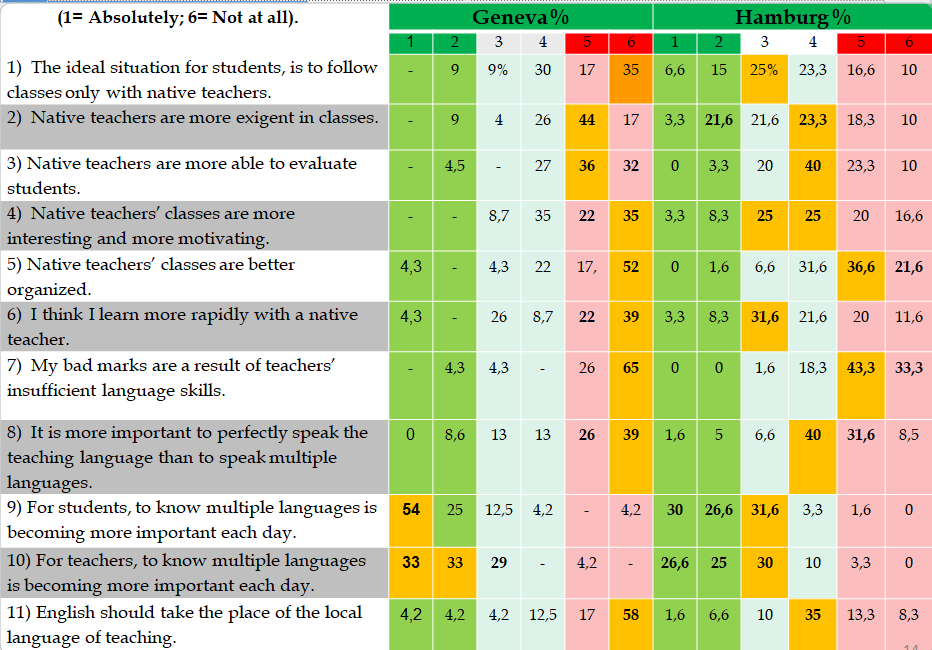
\includegraphics[width=\textwidth]{figures/Chapter9-img001.png}
% \caption{Observations on teachers’ language and teaching practices (1: I fully agree; 6: I don’t agree at all)\label{fig:9:1}}
%
% \todo[inline]{commas instead of decimal points?}
% \todo[inline]{why highlighting in font and bold and colour? (Row 10 for Geneva)}
% \todo[inline]{why percentages in Geneva 1:3 and Hamburg 1:3?}
% \todo[inline]{N.0 should be added to all bare Ns so that the precision is always one decimal digit}
% \todo[inline]{What is the difference between 0 and  --?}
% \todo[inline]{Why is 35 highlighted only once for question 4?}
%
% \end{figure}
\begin{figure}
\caption{Observations on teachers’ language and teaching practices (1: I fully agree; 6: I don’t agree at all)\label{fig:9:1}}

  \footnotesize
  \addfontfeatures{Numbers={Monospaced,Lining}}\selectfont
\begin{tabularx}{\textwidth}{@{}r@{~}>{\raggedright}p{3.5cm}@{~~} Y@{~}Y@{~}Y@{~}Y@{~}Y@{~}Y  | r@{~}Y@{~}Y@{~}Y@{~}Y@{~}Y@{}}
\lsptoprule
    &   &  \multicolumn{6}{c}{Geneva \%} &\multicolumn{6}{c}{Hamburg \%} \\
    \cmidrule(r){3-8}
    \cmidrule{9-14}
    &   & 1 & 2 & 3 & 4 & 5 & \multicolumn{1}{r}{6} & 1 & 2 & 3 & 4 & 5 & 6 \\
\midrule
1)  & The ideal situation for students is to follow classes only with native teachers.                    & 0 & 9.0 & 9.0 & 30.0 & 17.0 &  \highlight{35.0} & 6.6 & 15.0 & \highlight{25.0} & 23.3 & 16.6 & 10.0 \\
% \tablevspace
2)  & Native teachers are more exigent in classes.                                                        & 0 & 9.0 & 4.0 & \highlight{26.0} & 44.0 & 17.0 & 3.3 & 21.6  & 21.6 &\highlight{23.3} & 18.3 & 10.0\\
% \tablevspace
3)  & Native teachers are more able to evaluate students                                                  & 0 & 4.5 & 0 & 27.0 &\highlight{36.0} & 32.0 & 0 & 3.3 & 20.0 & \highlight{40.0} & 23.3 & 10.0\\
% \tablevspace
4)  & Native teachers' classes are more interesting and more motivating.                                  & 0 & 0 & 8.7 & \highlight{35.0} & 22.0 & \highlight{35.0} & 3.3 & 8.3 & \highlight{25.0} & \highlight{25.0} & 20.0 & 16.6\\
% \tablevspace
5)  & Native teachers' classes are better organized.                                                      & 4.3 & 0 & 4.3 & 22.0 & 17.0 &\highlight{52.0} & 0 & 1.6 & 6.6 & 31.6 &\highlight{36.6} & 21.6\\
% \tablevspace
6)  & I think I learn more rapidly with a native teacher.                                                 & 4.3 & 0 & 26 & 8.7 & 22.0 & \highlight{39.0} & 3.3 & 8.3 &\highlight{31.6} & 21.6 & 20.0 & 11.6\\
% \tablevspace
7)  & My bad marks are a result of teachers' insufficient language skills.                                & 0 & 4.3 & 4.3 & 0 & 26.0 & \highlight{65.0} & 0 & 0 & 1.6 & 18.3 &\highlight{43.3} & 33.3\\
% \tablevspace
8)  & It is more important to perfectly speak the teaching language than to speak multiple languages.     & 0 & 8.6 & 13.0 & 13.0 & 26.0 & \highlight{39.0} & 1.6 & 5.0 & 6.6 &\highlight{40} & 31.6 & 8.5\\
% \tablevspace
9)  & For students, to know multiple languages is becoming more important each day.                       &\highlight{54.0} & 25.0 & 12.5 & 4.2 & 0 & 4.2 & 30.0 & 26.6 & \highlight{31.6} & 3.3 & 1.6 & 0 \\
% \tablevspace
10) & For teachers, to know multiple languages is becoming more important each day.                       &\highlight{33.0} & \highlight{33.0} & 29.0 & 0 & 4.2 & 0 & 26.6 & 25.0 &\highlight{30.0} & 10.0 & 3.3 & 0 \\
% \tablevspace
11) & English should take the place of the local language of teaching.                                    & 4.2 & 4.2 & 4.2 & 12.5 & 17.0 &\highlight{58.0} & 1.6 & 6.6 & 10.0 &\highlight{35.0} & 13.3 & 8.3 \\
\lspbottomrule
\end{tabularx}
\end{figure}


\figref{fig:9:1} shows the results of quantitative data related to the evaluation of perceived classroom practices. The analysis of it makes clear that Swiss and Germans tend to position themselves differently regarding the way the sentences are formulated (see highlights in yellow). Thus, Swiss students tend to answer either positively or negatively at the extreme end of the scale (positions 1 or 6), while German students seem to be more cautious and tend to position themselves on neutral values of the scale (positions 3 and 4). These different positions may be explained by the linguistic diversity of the class population. On the Geneva side, 25.8\% of the respondents have two first languages, 36.6\% declare trilingual; 20\% speak four languages, 10\% are pentalingual, 13.3\% sextalingual, 3.3\% septalingual and the same percentage octalingual. On the German side, students declare themselves mostly as German (41 out of 60) and having German as a mother tongue (55 out of 60).

The choice to have only native teachers was rejected by a large percentage of respondents: 49.9\% (UH) and 82\% (UGE), respectively. Among the justifications given was that it would interrupt interculturality; it would be a shame to miss out on very good teachers, especially since “a nonnative can have the same abilities to teach as a native” (UGE). Some students are of the opinion that “diversity is always a linguistic and cultural richness” (UGE). At this point, according to these students, nonnative teachers are more comfortable with cultural differences, more likely to help students to deal with them, and to share their own culture and to step out of their comfort zone (\citealt{Pratt1991}; \citealt{Yanaprasart2017}).

\begin{quote}
With a nonnative teacher, I think there are also cultural aspects. S/he also learned the cultural aspects of the teaching language. (UGE\_9)
\end{quote}

\begin{quote}
Well, good, also there, that (s)he has perhaps other perspectives, isn’t it?  As someone who is representative of the culture him/herself. /Ähm/ perhaps is (s)he more objective, perhaps not, I don’t really know. Perhaps there is not such a thing as objectivity. But well (..) another perspective and (s)he has also perhaps more experience regarding intercultural encounters. (UH\_3)
\end{quote}

The interesting thing underlined by the interviewed students is about diversity: a diversity that comes to “us”, which can open the mind to different points of view and perspectives. If it is very good to have cultural references from local teachers, having expatriate teachers should be encouraged so as to have contacts with different accents and intercultural experiences. Diversity is a synonym for richness, and mixing means force and dynamic. A mixed team should be created, and a balanced collaboration between local and international teachers should be encouraged and optimized: “I like the mixing of teachers. Diversity of teachers signifies richness. For me, it’s something positive.” (UGE\_4) 

Furthermore, while Swiss students do not tend to perceive native teachers as more interesting, motivating or better organized, German students tend to perceive these characteristics as not being necessarily attached to the linguistic skills, but more skeptically: regarding the need to perfectly master the language, a German student states that correctness is “not necessary for transmitting content” and that “we learn from errors” (from anonymous questionnaire).  In both cases, however, organization is not perceived as being particularly attached to the native teacher. Regarding the question of the organization of courses, the vast majority of respondents believe that good organization “has nothing to do with being native”. On the other hand, it seems to them that “nonnative teachers make more efforts” to organize their courses. Additionally, just a small number of respondents agree with the finding that native teachers are more demanding in class, in both contexts. But again, some divergences emerge: while, for some interviewees, the requirements are the same, for others, it is quite the opposite: it is nonnative teachers who are more demanding. As for a third group of remarks, the requirement does not depend on the origin of the teacher, it depends on character.

Also different is the positioning of German and Swiss students regarding their perception of degree of requirement and the ability to evaluate students. While Swiss students do not envisage such a relationship, German students, again, are quite undecided and avoid a clear positioning. When asked about the assessment skills, all respondents think that both categories of teachers have the same abilities. Indeed, “the ability to evaluate does not depend on the language of instruction”, wrote one respondent. “It’s not an ability related to language proficiency”, argues another from the same institution. Nevertheless, many more Swiss than German students are willing to attest that their grades do not depend on teachers’ linguistic skills. Another interesting feature concerns the different assessment of rapidity of learning with native speakers: while the majority of the Swiss students (61\%) answer that they do not learn easier and more rapidly with native speakers, German students position themselves again in the middle values, which leaves some place for thoughts on the impact of comprehensiveness of teachers’ input into their cognitive work in the classroom. So, having classes with nonnative speakers may be perceived as delaying the acquisition of content, at least from the perspective of the inquired German students.

The majority of the surveyed students share the opinion about the importance of the “perfect mastery” of the language of instruction. It is important to note that, in both universities, in order to deconstruct stereotypes about being bilingual or plurilingual, students stress the impact of explicit instruction acquired in the classroom about bilingualism and “partial” linguistic proficiency: 

\begin{quote}
I have always thought that being bilingual means speaking perfectly two languages at the same level, but it is not, in fact not necessarily. Anyway, we always learn a language, even our own mother tongue; we will continue to learn until we die. (UGE\_5)
\end{quote}

\begin{quote}
I would really like to speak as a native speaker, I would really love it a lot, I guess, that it is very / very difficult to attain, I don’t know. /ahm/ but, yes, the time spent in my university had had an influence on me – and it is perhaps good so – the time at the university had shown me that is not necessary [to speak like a native speaker], and I had this impression previously (laughs). (UH\_3) 
\end{quote}

To the question of whether it is more important to speak the language of teaching perfectly than to speak several languages (sentence 8), certain diversity in the answers can be observed. If no one answered “absolutely”, 21.6\% said “yes” and “rather yes”. It is the “absolutely”, “yes” and “rather yes” answers that win in the following two observations in both contexts: knowing several languages is more and more important for students and speaking several languages is more and more important for teachers (sentences 9 and 10). On the learners’ side, it has been shown that “it is an undeniable wealth; an asset for life; an advantage in our present society; for certain mobility; for studies; to read articles, books written in a foreign language” (UGE). With regard to teachers, the fact that they must “work with foreign colleagues, or even with foreign universities, they need to speak several languages” (UGE). More precisely, plurilingual resources are “vital for acquiring and transmitting knowledge” (UGE). But, even if plurilingual skills are perceived as very positive from both sides, German students are less effusive regarding this optimistic evaluation. This cautious position may be correlated with the answers to question 8: more German than Swiss students are skeptical regarding the sentence “It is more important to perfectly speak the teaching language than to speak multiple languages”, meaning that the plurilingual competence is less positively evaluated than mastering perfectly the language of instruction. 

For the last question of whether the English language should replace the local language, it is the answer “rather not” that wins most of the German answers, with 35\%, while on the Swiss side, the answers are “rather not” at 12.5\%, “no” at 17\% and “not at all” at 58\%. Note that at the University of Geneva, the French language is the main language of instruction for all subjects within the bachelor degree. A passive or good knowledge – in a second language, in this case in English – is recommended or even necessary to study. That is to say, most disciplines recommend or require knowledge in several languages: 78.57\% for university baccalaureates and 69\% for master’s degrees. This requirement reflects a desire to maintain the local language while allowing the integration of an international dimension in curricula.\footnote{At the University of Geneva, half of 71 disciplines for the master degree (52.11\%) require knowledge of two languages: French-English (81.08\%), English-French (18.91\%); 14.08\% (French); 11.26\% (English); 19.71\% (Trilingual): French-English-German (6 masters), German-French-English (5 masters), French-English-combined languages (3 masters). No such requirements exist in Hamburg, except for Bachelor and Master studies, related, for example, to foreign language teaching.} We may say that this university language policy has a certain impact on the students’ perceptions towards the role and place of English in the study program.

\section{Discussion and concluding remarks}

In light of the foregoing, students do not report any significant superiority of “nativism” between the two groups of teachers. In addition, most respondents are of the opinion that there is no relationship between the way of teaching and the language skills of the teacher. Furthermore, no difference is perceived in evaluation practices. What students expect from their teachers in both categories is that they are able to make the learning process relevant and motivating, that they are sensitive and responsive to student needs, and finally are able to respect their learners as individuals with their own aspirations.

If there is a difference, it concerns more a cultural than a linguistic aspect. It is about a question of personality: “it is more related to the person and to his pedagogical sensitivity than to the mother tongue”. Unlike Medgyes’ conclusion (\citeyear{Medgyes1992,Medgyes1994}), according to which the difference between native and nonnative teachers from the point of view of the teachers interviewed comes mainly from language competence, at least in the field of foreign language teaching, our sample is of the opinion that no one is better than anyone because of his/her linguistic competence, but by reason of his/her professional, didactic and pedagogical skills. A difference would be mainly in the way of transmitting knowledge, as one student said: “It’s not enough to be a native speaker but you have to know how to teach” (UGE). For \citet[104]{Bento2011}, both linguistic skills (the knowledge of “describing” language-culture) and teaching skills (the knowledge to “transmit” in a given context) are necessary. While the results of Medgyes’ research (\citeyear{Medgyes1992,Medgyes1994}) in the field of foreign language teaching reveal that language competence is the main cause of the different ways of teaching native and nonnative teachers, none of our responses shows a correlation between way of teaching and linguistic competence, and this across different disciplinary fields. According to Medgyes, this difference in his study does not necessarily imply that a nonnative does not teach as well as a native, because the former finds effective teaching strategies to compensate for his/her possible linguistic weaknesses. 

To this point, the students’ perception of the ability of L1 teachers to use the language “naturally” may explain why they are portrayed as having shown more confidence in their skills, particularly in grammar, conversation and pronunciation, and were specifically appreciated for their knowledge in the culture of the language taught. Nonnative teachers have been described as experienced and understandable as having lived the same trajectory, which seems to be positive and encouraging for learners who aspire to follow in their footsteps, portrayed as an accessible and feasible model from a professional perspective. \citet[46]{Castellotti2011} talks about an enhancement of approximation, linking, circumvention and transfer capabilities (our translation). By learning with teachers whose conditions are close to their own, these students hope to acquire the same skills. By means of their plurilingual resources acquired and by plurilingual pedagogical practices, teachers learn to build up translinguistic and intercultural strategies while promoting a dynamic vision of language competence, as well as intercultural awareness when teaching in multicultural and multilingual classes. So, learners and teachers develop reflexive and critical skills side by side.

The main comparative differences across the two contexts are located at the perception of the “plurilingual nonnativism”. The plurilingual teacher is observed with more enthusiasm and acceptance on the Swiss side than on the German side, which views with more caution the advantages of having nonnative teachers and the understanding of the plurilingual repertoires as partial linguistic skills. As a matter of fact, in regard to the Hamburg side, the findings suggest two main points: 

\begin{enumerate}
\item a very high permeability to normative and less plurilingual ideologies (“[…] well, we really try to express ourselves as a native speaker. It is a somehow the norm”); and 
\item the “invisibility” of the plurilingual nonnative speaker. 
\end{enumerate}

\noindent Terms such as \emph{native} and \emph{nonnative}, as well as \emph{norm} and \emph{correctness}, consistently emerge as heuristic categories in the German interviews. Concerning the Geneva students, their answers suggest a firm and favorable position to plurilingualism. Teachers’ competences are not evaluated in terms of being a native or nonnative teacher, but instead of as being able to speak one, two or more languages \citep{Bento2011}. Partial skills in multiple languages are positively portrayed. As such, the diversity of teachers’ linguistic repertoires represents cognitive, pedagogical, communicative and didactic resources and strategies.

Taking the above into account, in the eyes of the surveyed students, teachers’ plurilingual skills potentially represent, in terms of knowledge acquisition and transmission, an “added value”, an undeniable strength and an inescapable advantage to impart knowledge in a multilingual and multicultural classroom, if only they feel prepared to do it. Otherwise, a “partial” linguistic proficiency is just a “mudded” value since most of the time students and teachers abide by the monolingual and monoglossic habitus of the educative institutions (mainly in the German context). So, if as mentioned by \citet{Cook1991,Cook2008}, the knowledge of two or more languages in one mind contributes considerably to the quality of teaching\slash learning in terms of motivation and cognitive development, these advantages should be more thematized, developed and discussed, particularly in language learning classrooms and in teaching education practices and supervision. The challenge for institutions is to change the environment by changing the perception of “language-as-problem” or “language-as-right” to “language-as-resource” \citep{Ruiz1984}.

In light of these reflections, it is especially in a transformative \citep{SavinBaden2008}  “troublesome space” \citep{Montgomery2011} that the “monolingual habitus” \citep{Gogolin2008} leaves its place to the “plurilingual mind” \citep{Menghini2017}, where the use of a language can occur not as a simple, fixed and rigid code, but as a complex, yet flexible, dynamic and evolving tool so as to better explore knowledge in the service of learning quality \citep{Berthoud2016}. A diversification of knowledge will be optimal in an environment where different cultures and languages have the opportunity to interact in a hybrid and multilateral perspective \citep{Yanaprasart2018}, thus constituting a rewarding model of inspiration to open up to global knowledge.

{\sloppy\printbibliography[heading=subbibliography,notkeyword=this]}
\end{document}
